% lecture06.tex — Sard's Theorem

\section{Sard's Theorem}

\begin{theorem}{Sard's Theorem}{sard}
    Let $f \colon M \to N$ be a smooth map, and let
    \[
        C = \{x \in M \mid \rank\, df_x < \dim N\}
    \]
    be the set of critical points. Then, the set of critical values, $f(C)$, has measure zero in $N$.
\end{theorem}

\begin{proof}
    Thanks to second-countability of manifolds, it suffices to prove it for $f \colon U \to \R^p$, $U \overset{\text{open}}{\subset} \R^n$.

    We proceed by induction on $n$. Note, it is trivial for $n = 0$.

    Let
    \[
        C_1 = \{x \in U \mid df_x = 0\}
    \]
    and more generally
    \[
        C_k = \left\{x \in U \;\middle|\; \frac{\partial^j f}{\partial x_{s_1} \cdots \partial x_{s_j}}(x) = 0 \text{ for all } j \leq k \text{ and } 1 \leq s_1, \ldots, s_j \leq n\right\}.
    \]
    Thus we have a descending sequence of closed sets
    \[
        C \supset C_1 \supset C_2 \supset \cdots.
    \]

    We will prove the theorem in three steps:

    \textbf{Step 1:} $f(C - C_1)$ has measure zero.

    \textbf{Step 2:} $f(C_k - C_{k+1})$ has measure zero, for $k \geq 1$.

    \textbf{Step 3:} $f(C_k)$ has measure zero for $k$ sufficiently large.

    \begin{proof}[Proof of Step 1]
        We may assume $p \geq 2$, since $C = C_1$ when $p = 1$.

        We will use:
        \begin{theorem}{Fubini}{fubini}
            A measurable set $A \subset \R^p = \R \times \R^{p-1}$ must have measure zero if it intersects each hyperplane $(\text{const.}) \times \R^{p-1}$ in a set of $(p-1)$-dimensional measure zero.
        \end{theorem}

        For each $x \in C - C_1$, we will find an open neighborhood $V \subset \R^n$ so that $f(V \cap C)$ has measure zero.

        Since $x \notin C_1$, some partial derivative, say $\frac{\partial f_1}{\partial x_1}$, is nonzero at $x$. Consider the map $h \colon U \to \R^n$,
        \[
            x \mapsto (f_1(x), x_2, \ldots, x_n).
        \]
        Since $dh_x$ is nonsingular, it is a local diffeomorphism; it maps some neighborhood $V$ of $x$ diffeomorphically on to an open set $V' \subset \R^n$.

        \begin{center}
        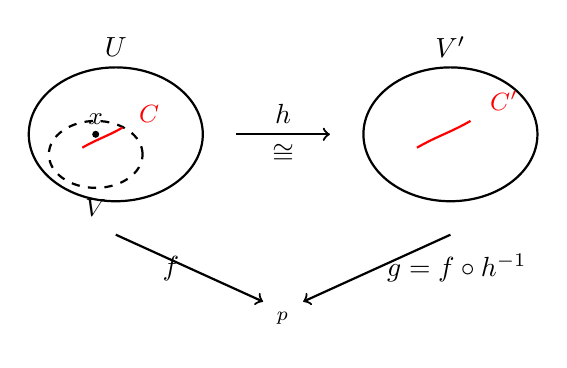
\begin{tikzpicture}[scale=0.85]
            % U with V, C
            \draw[thick] (0,0) ellipse (1.3 and 1);
            \node at (0,1.3) {$U$};
            \draw[thick,dashed] (-0.3,-0.3) ellipse (0.7 and 0.5);
            \node at (-0.3,-1.1) {\small $V$};
            \fill (-0.3,0) circle (1.5pt) node[above] {\small $x$};
            \draw[thick,red] (-0.5,-0.2) to[out=30,in=210] (0.1,0.1);
            \node[red] at (0.5,0.3) {\small $C$};
            % Arrow h
            \draw[->,thick] (1.8,0) -- (3.2,0) node[midway,above] {$h$} node[midway,below] {$\cong$};
            % V' with C'
            \draw[thick] (5,0) ellipse (1.3 and 1);
            \node at (5,1.3) {$V'$};
            \draw[thick,red] (4.5,-0.2) to[out=30,in=210] (5.3,0.2);
            \node[red] at (5.8,0.5) {\small $C'$};
            % Arrow f, g
            \draw[->,thick] (0,-1.5) -- (2.2,-2.5) node[midway,left] {$f$};
            \draw[->,thick] (5,-1.5) -- (2.8,-2.5) node[midway,right] {$g = f \circ h^{-1}$};
            \node at (2.5,-2.8) {$\R^p$};
        \end{tikzpicture}
        \end{center}

        Set $g := f \circ h^{-1}$. Then the set $C'$ of critical points of $g$ is $h(V \cap C)$, and the set $g(C')$ of critical values of $g$ is $f(V \cap C)$.

        Note, $g$ carries hyperplanes into hyperplanes; let
        \[
            g^t \colon (t \times \R^{n-1}) \cap V' \to t \times \R^{p-1}
        \]
        denote the restriction of $g$. Moreover, since
        \[
            \left(\frac{\partial g_i}{\partial x_j}\right) = \begin{pmatrix} 1 & 0 \\ * & \frac{\partial g^t_i}{\partial x_j} \end{pmatrix},
        \]
        a point of $t \times \R^{n-1}$ is critical for $g^t$ iff it is critical for $g$.

        By induction hypothesis, the set of critical values of $g^t$ has measure zero in $t \times \R^{p-1}$. Hence, by Fubini's theorem, the set
        \[
            g(C') = f(V \cap C)
        \]
        has measure zero, which completes Step 1.
    \end{proof}

    \begin{proof}[Proof of Step 2]
        (Similar to Step 1.)

        For each $x \in C_k - C_{k+1}$, some $(k+1)$-st derivative is nonzero, so let's say $w(x) = \frac{\partial^k f_r}{\partial x_{s_1} \cdots \partial x_{s_k}}$ vanishes at $x$ but $\frac{\partial w}{\partial x_1}$ does not.

        Then the map $h \colon U \to \R^n$, $x \mapsto (w(x), x_2, \ldots, x_n)$, carries some neighborhood $V$ diffeomorphically onto an open set $V' \subset \R^n$.

        Note, $h$ carries $C_k \cap V$ into the hyperplane $0 \times \R^{n-1}$. Hence, we can consider $g := f \circ h^{-1} \colon V' \to \R^p$ and its restriction $\bar{g} \colon (0 \times \R^{n-1}) \cap V' \to \R^p$.

        By induction, the set of critical values of $\bar{g}$ has measure $0$ in $\R^p$, and in particular, $\bar{g} \circ h(C_k \cap V) = f(C_k \cap V)$ has measure zero.
    \end{proof}

    \begin{proof}[Proof of Step 3]
        Let $I^n \subset U$ be a cube with edge $\delta$. We will prove that if $k$ is sufficiently large, $f(C_k \cap I^n)$ has measure zero. (The constant depends only on $f$ and $I^n$.)

        By Taylor's theorem, $f(x + h) = f(x) + R(x,h)$ where $\|R(x,h)\| \leq c\|h\|^{k+1}$ for $x \in C_k \cap I^n$, $x + h \in I^n$.

        Now, subdivide $I^n$ into $r^n$ cubes of edge $\frac{\delta}{r}$.

        Then, for each cube $I'$ in the subdivision containing a point $x \in C_k$, any other point of $I'$ can be written as $x + h$ with $\|h\| \leq \sqrt{n}\,\frac{\delta}{r}$, so
        \[
            \operatorname{Volume}(f(C_k \cap I')) \leq \left(2c\left(\sqrt{n}\,\frac{\delta}{r}\right)^{k+1}\right)^p.
        \]
        Therefore,
        \[
            \operatorname{Volume}(f(C_k \cap I^n)) \leq r^n \cdot \left(2c\left(\sqrt{n}\,\frac{\delta}{r}\right)^{k+1}\right)^p = c' \cdot r^{n - (k+1)p}
        \]
        which holds for any $r \in \Z_{>0}$, so we can send $r \to \infty$. And hence if $k + 1 > \frac{n}{p}$, $f(C_k \cap I^n)$ must have measure zero.

        This completes the proof of Sard's theorem.
    \end{proof}
\end{proof}
